\documentclass[tikz, border=5pt]{standalone}
\usepackage{pgfmath}

\begin{document}
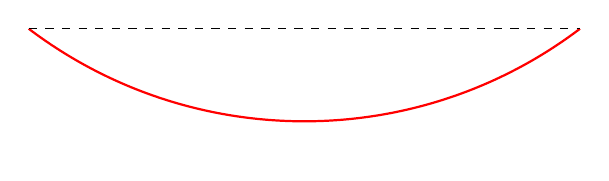
\begin{tikzpicture}

  % Khai báo bằng pgfmathsetmacro để đảm bảo là số thực
  \pgfmathsetmacro{\R}{5.8}
  \pgfmathsetmacro{\s}{3.5}

  % Tính góc chắn cung (đơn vị độ)
  \pgfmathsetmacro{\angle}{2 * asin(\s / \R)}

  % Vẽ cung tròn đối xứng qua Oy
  \draw[thick, red]
    ({270-\angle/2}:\R) arc[start angle={270-\angle/2}, end angle={270+\angle/2}, radius=\R];

  % Vẽ dây cung
  \draw[dashed]
    ({270-\angle/2}:\R) -- ({270+\angle/2}:\R);

  % Ghi chú thông tin
%   \node at (0,-0.5) 
%     {$R = \pgfmathprintnumber{\R}$ cm,\quad 
%       $s = \pgfmathprintnumber{\s}$ cm,\quad 
%       $\theta \approx \pgfmathprintnumber[fixed, precision=2]{\angle}^\circ$};

\end{tikzpicture}
\end{document}
